\subsection{Optimized Similarity Rules (RQ5)}
\label{sec:res:opt}

Table~\ref{tab:optsummary} and Fig.~\ref{fig:optgain} compare the optimized similarity policy with the default policy and with the best fixed policy on the \Reps{} test replications. For the access objective the optimized policy lowered RATP by \OptAccessGainDefaultMean\% relative to the default on average (up to \OptAccessGainDefaultMax\%) and by \OptAccessGainBestMean\% relative to the best fixed policy (between \OptAccessGainBestMin\% and \OptAccessGainBestMax\%). For the balanced objective the corresponding improvements were \OptBalancedGainDefaultMean\% (up to \OptBalancedGainDefaultMax\%) and \OptBalancedGainBestMean\% (between \OptBalancedGainBestMin\% and \OptBalancedGainBestMax\%). The optimized policy was significantly better than the best fixed policy in \OptAccessNSigBetter{} (access) and \OptBalancedNSigBetter{} (balanced) of the \NEdTypes{} ED types and significantly worse in none. The comparison favours the fixed policies, which are selected on the test replications that the optimized policy never saw.

\begin{table*}[!htbp]
\centering
\caption{Improvement (\%) of the optimized similarity policy in its objective over the default policy and over the best fixed policy, averaged over the three load levels (\Reps{} test replications). Better/worse: number of load levels in which the paired 95\% confidence interval of the difference from the best fixed policy excludes zero.}
\label{tab:optsummary}
\footnotesize
\begin{adjustbox}{max width=\linewidth}\begin{tabular}{llrrrrrr}
\toprule
 & & \multicolumn{3}{c}{Access objective (RATP)} & \multicolumn{3}{c}{Balanced objective} \\
\cmidrule(lr){3-5}\cmidrule(lr){6-8}
Acuity mix & Configuration & vs default & vs best fixed & Better/worse & vs default & vs best fixed & Better/worse \\
\midrule
Tertiary & Pooled & 14.4 & 3.5 & 3/0 & 8.8 & 1.2 & 1/0 \\
 & Fast track & 23.0 & 3.2 & 2/0 & 13.8 & 1.2 & 2/0 \\
 & Split flow & 25.5 & 16.0 & 3/0 & 10.3 & 3.4 & 3/0 \\
Community & Pooled & 8.9 & 2.3 & 1/0 & 6.2 & 1.2 & 1/0 \\
 & Fast track & 21.8 & 4.3 & 2/0 & 11.9 & 2.5 & 2/0 \\
 & Split flow & 29.0 & 22.1 & 3/0 & 13.2 & 8.2 & 3/0 \\
Urgent-care-like & Pooled & -0.6 & -3.6 & 0/0 & 2.0 & -1.3 & 0/0 \\
 & Fast track & 31.5 & 8.1 & 2/0 & 19.6 & 4.0 & 1/0 \\
 & Split flow & 41.4 & 36.0 & 3/0 & 20.4 & 16.9 & 3/0 \\
\bottomrule
\end{tabular}\end{adjustbox}
\end{table*}

\begin{figure*}[!htbp]
\centering
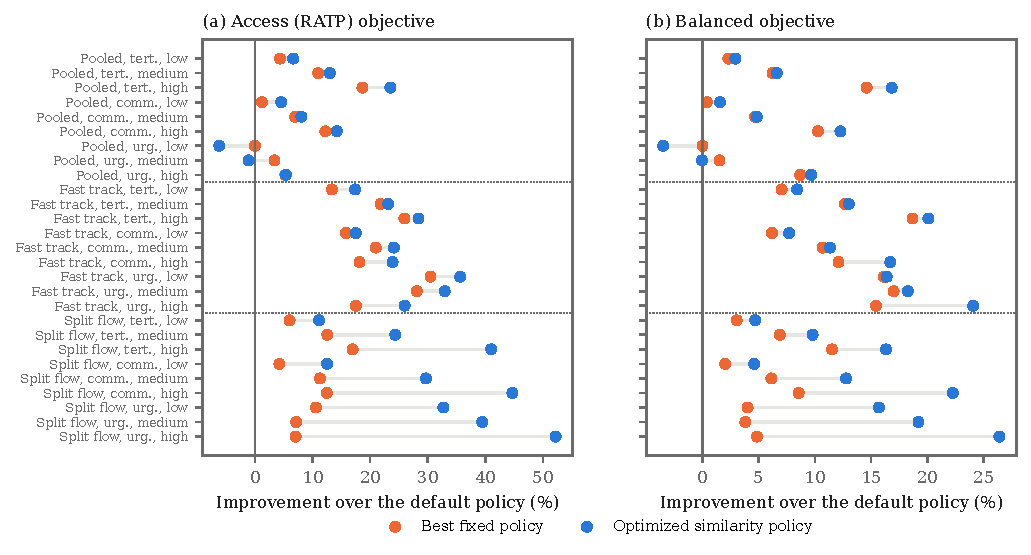
\includegraphics[width=0.95\figtw]{figures/fig_opt_gain.pdf}
\caption{Improvement over the default policy of the best fixed policy and of the optimized similarity policy, by ED type and objective (\Reps{} test replications). ED types are grouped by configuration.}
\label{fig:optgain}
\end{figure*}

The gain depends mainly on the configuration. In pooled EDs, where only the queue rule can be changed, the optimized policy improved on the best fixed policy by \OptAccessGainBestPooled\% (access) and \OptBalancedGainBestPooled\% (balanced) on average; in the pooled urgent-care-like EDs at low and medium load it did not find a better rule than the fixed CTAS-based rules, and the small differences were not significant. In fast-track EDs the gains were \OptAccessGainBestFasttrack\% and \OptBalancedGainBestFasttrack\%, and in split-flow EDs \OptAccessGainBestSplitflow\% and \OptBalancedGainBestSplitflow\%. The large gains in split-flow EDs come from routing. The optimized routing offsets were negative in \OptBalancedNOffsetNeg{} of the \OptBalancedNTwoArea{} two-area ED types (balanced objective), so the optimized rules send more patients to the second area than similarity routing does: in split-flow EDs \OptBalancedShareSecondSplitOpt\% of patients on average, against \OptBalancedShareSecondSplitBest\% under the best fixed policy and \OptBalancedShareSecondSplitDefault\% under the default. As in Section~\ref{sec:res:mech}, the fixed routing rules leave second-area capacity unused, and a tuned threshold uses more of it.

Fig.~\ref{fig:optparams} shows the optimized parameters for the balanced objective (access: Appendix~\aref{app:res:opt}). Four regularities stand out.

First, the optimized rules are not lexicographic in CTAS. The lexicographic condition (\ref{eq:lexcond}) held for attribute A in \OptAccessNLexA{} (access) and \OptBalancedNLexA{} (balanced) of the \NEdTypes{} optimized rules, so apart from CTAS~1, which is always served first, a less urgent patient can be seen before a more urgent one when the other attributes favour it. The median weight on CTAS was \OptBalancedWAMedian{} (balanced).

Second, the rules move toward short service as load increases. The service-class target was the shortest class ($q_B=5$) in \OptBalancedNqBFive{} of the balanced rules. At high load the weight on service class exceeded the weight on CTAS in \OptBalancedNWbGtWaHigh{} of the nine ED types (median $w_B=\OptBalancedWbMedianHigh$), at low load in \OptBalancedNWbGtWaLow{} (median $w_B=\OptBalancedWbMedianLow$). This is the logic of index rules of the $c\mu$ type \cite{VanMieghem1995_GenCMu,Mandelbaum2004_GenCMu}: when queues are long, serving short patients first reduces the number waiting, and the optimization trades some acuity order for this effect. It also shortened the longest waits of the least urgent patients: the median ratio of the 95th percentile of door-to-physician time of CTAS~5 patients under the optimized and the best fixed policy was \OptBalancedCtasFiveTailRatio{} (balanced), while the same ratio for CTAS~2 was \OptBalancedCtasTwoTailRatio.

Third, the reassessment bonus depends on the objective. Under the access objective $\beta$ was negative in all \OptAccessNBetaNeg{} ED types (median \OptAccessBetaMedian), so new patients were seen before patients waiting for reassessment. Under the balanced objective $\beta$ was negative in \OptBalancedNBetaNegLowMed{} of the \OptBalancedNLowMed{} ED types at low and medium load but positive in \OptBalancedNBetaPosHigh{} of the nine at high load, where length of care weighs most. This agrees with Shakeri et al.\ \cite{Shakeri2025_WhoToSeeNext}: in-progress patients first when the length of care matters, new patients first when their waiting time is the main concern. The access objective illustrates the risk of optimizing access alone: it reached its RATP partly by delaying reassessments, and mean LOS under the access-optimized rule was up to \OptAccessLosChangeMax\% higher than under the best fixed policy, whereas under the balanced objective it stayed within \OptBalancedLosChangeMax\% in every ED type.

Fourth, the optimized ageing rates were close to zero. Because the search started from the SIM rule, which has no ageing, it sampled large ageing rates rarely, so we re-ran every optimized rule with fixed ageing rates between \LeverGammaMin{} and \LeverGammaMax{} (experiment E6b, \NLeverReps{} test replications; Table~\aref{tab:levers}). Ageing made the rules worse on average at every rate, by \LeverBalancedGammaBestMean\% at the smallest rate and \LeverBalancedGammaLargeMean\% at the largest under the balanced objective, and improved them by more than 1\% in at most \LeverBalancedGammaNBetter{} ED types. For these objectives ageing does not help. The same check shows which parameters carry the gain. Setting the reassessment bonus to zero worsened the access objective by \LeverAccessBetaZeroMean\% on average (worse by more than 1\% in \LeverAccessBetaZeroNWorse{} ED types) but the balanced objective by only \LeverBalancedBetaZeroMean\%. Removing the routing offset worsened the two objectives by \LeverAccessOffsetZeroMean\% and \LeverBalancedOffsetZeroMean\% on average and by up to \LeverAccessOffsetZeroMax\% and \LeverBalancedOffsetZeroMax\%.

\begin{figure*}[!htbp]
\centering
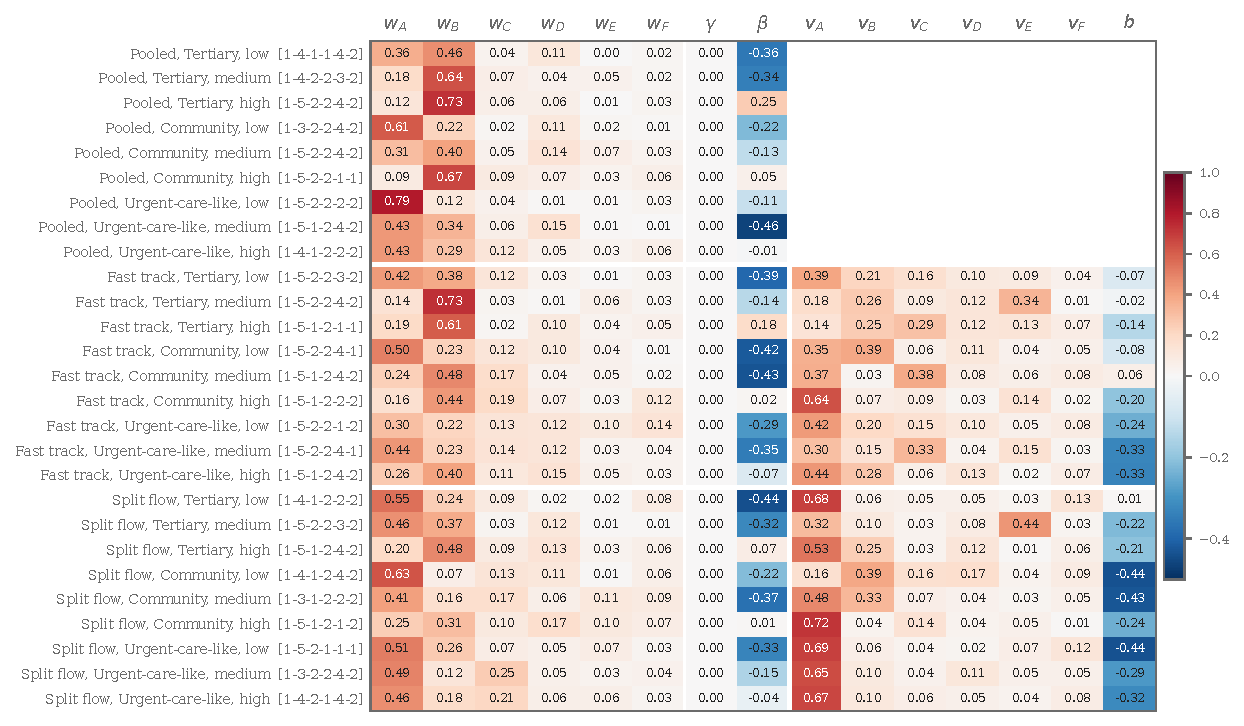
\includegraphics[width=0.9\textwidth]{figures/fig_opt_params_balanced.pdf}
\caption{Parameters of the similarity rules optimized for the balanced objective. Rows: ED types, with the optimized target code $q_A$--$q_F$ in brackets. Columns: queue weights $w_A$--$w_F$, ageing $\gamma$, reassessment bonus $\beta$, routing weights $v_A$--$v_F$ and routing offset $b$ (two-area EDs only).}
\label{fig:optparams}
\end{figure*}

\paragraph*{Transfer} Fig.~\aref{fig:transfer} reports the transfer regret of every optimized rule in every other ED type of the same configuration (\TransferBalancedNPairs{} pairs per objective). Most rules transferred well: the median regret was \TransferBalancedMedian\% under the balanced objective and \TransferAccessMedian\% under the access objective, and the regret was below 5\% in \TransferBalancedShareUnderFive\% and \TransferAccessShareUnderFive\% of the pairs. Rules transferred better between ED types with the same acuity mix (mean regret \TransferBalancedSameAcuity\%, balanced) than between acuity mixes (\TransferBalancedOtherAcuity\%). The exceptions are concentrated in one ED type. In the \TransferBalancedWorstTarget{} ED, \TransferBalancedNOverFiftyWorstTarget{} rules optimized elsewhere had a balanced regret above \TransferBigRegret\% (up to \TransferBalancedMax\%): their routing thresholds sent more patients to the second area than its capacity could absorb in an ED with many admitted patients and little spare capacity. A tightly loaded split-flow ED therefore needs a rule tuned to its own capacity split. Within each configuration, the single donor rule with the smallest mean regret over the other ED types had a mean balanced regret of \TransferBalancedDonorMean\% and a maximum of \TransferBalancedDonorMax\%, so a health system could share one rule per configuration at a modest loss.

\subsection{Robustness and Out-of-Sample ED Types}
\label{sec:res:robust}

Under misspecified inputs (E8, Table~\aref{tab:rob} in Appendix~\aref{app:res:rob}), the ranking of the fixed policies changed little. The mean Kendall $\tau$ between the ranking under the perturbed and the core inputs was \RobTauRatpMean{} for RATP (lowest variant \RobTauRatpMin) and \RobTauLosMean{} for mean LOS (lowest \RobTauLosMin). The policy that was best under the core inputs remained best for RATP in \RobSameBestRatp\% of the cases; its regret under the perturbed inputs was \RobRegretRatpMean\% on average and at most \RobRegretRatpMax\% for RATP, and at most \RobRegretLosMax\% for mean LOS. The rule optimized for the balanced objective under the core inputs, used under the perturbed inputs, differed from the best fixed policy under those inputs by \RobOptVsBestMean\% on average (negative values: the optimized rule is better; worst case \RobOptVsBestMax\%) and remained \RobOptGainDefaultMean\% better than the default.

\begin{figure}[!htbp]
\centering
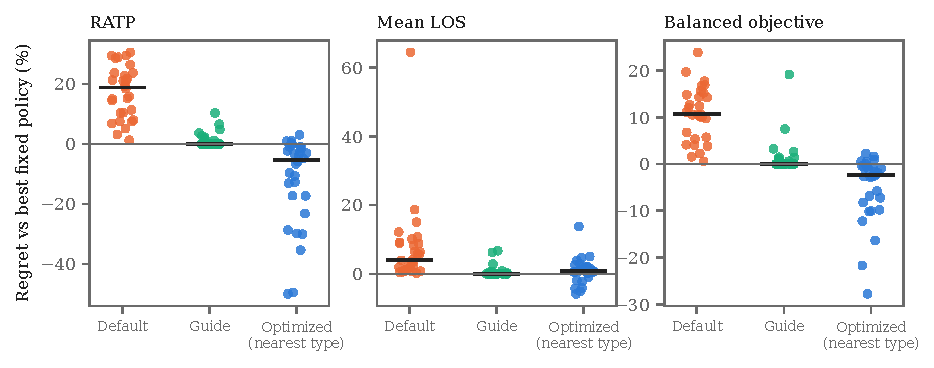
\includegraphics[width=\figcw]{figures/fig_oos.pdf}
\caption{Regret relative to the best fixed policy in \NOosTypes{} out-of-sample ED types (E9, \NOosReps{} replications) of the default policy, the policy recommended by the decision guide for the nearest acuity mix and the same configuration, and the rules optimized for the nearest core ED type (access rule for RATP, balanced rule otherwise). Horizontal lines: medians.}
\label{fig:oos}
\end{figure}

In the \NOosTypes{} out-of-sample ED types of E9 (\OosVisitsMin--\OosVisitsMax{} visits per day), the decision guide, applied with the nearest acuity mix and the ED's configuration, had a mean regret of \OosGuideRatpMean\% for RATP and \OosGuideLosMean\% for mean LOS, against \OosDefaultRatpMean\% and \OosDefaultLosMean\% for the default policy (Fig.~\ref{fig:oos}). The regret of the guide exceeded 10\% for RATP in \OosGuideRatpNGtTen{} of the \NOosTypes{} ED types, that of the default in \OosDefaultRatpNGtTen. The rules optimized for the nearest core ED type did better than any fixed policy on average: their mean regret relative to the best fixed policy was \OosOptRatpMean\% for RATP (access rule) and \OosOptBalMean\% for the balanced objective (balanced rule), and at most \OosOptRatpMax\% and \OosOptBalMax\%. The guide and the optimized rules therefore carry over to ED types between the design points, which is the situation of an ED that uses them without its own model.
